\documentclass{article}

\usepackage{onecolceurws}

\usepackage{url}
\usepackage{xspace}
\usepackage{xparse}
\usepackage{color}
\usepackage{amsmath, amsfonts, amssymb}
\usepackage{stmaryrd}
\usepackage{mathrsfs}
\usepackage{array}
\usepackage{enumitem}
\usepackage{endnotes}
\usepackage{hyperref}
\usepackage{bussproofs}
\usepackage{subcaption}
\usepackage{stackengine}

\usepackage{marvosym}

\def\B{\mathcal{B}}
\def\C{\mathcal{C}}
\def\D{\mathcal{D}}
\def\E{\mathcal{E}}
\def\F{\mathcal{F}}
\def\G{\mathcal{G}}
\def\I{\mathcal{I}}
\def\L{\mathcal{L}}
\def\M{\mathcal{M}}
\def\O{\mathcal{O}}
\def\P{\mathcal{P}}
\def\Q{\mathcal{Q}}
\def\R{\mathcal{R}}
\def\S{\mathcal{S}}
\def\T{\mathcal{T}}
\def\U{\mathcal{U}}
\def\V{\mathcal{V}}
\def\W{\mathcal{W}}
\def\X{\mathcal{X}}

\def\Cf{\mathfrak{C}}
\def\Df{\mathfrak{D}}
\def\Ifr{\mathfrak{I}}
\def\Sf{\mathfrak{S}}


\newcommand{\dom}{\mathit{dom}}
\newcommand{\ran}{\mathit{ran}}
\newcommand{\FV}{\text{FV}}

\newcommand{\lang}{\mathscr{L}}

\newcommand*\red[1]{\textcolor{red}{#1}}
\newcommand*\blue[1]{\textcolor{blue}{#1}}

%%% Local Variables:
%%% mode: latex
%%% TeX-master: t
%%% End:

\usepackage{xspace}
\usepackage{mathtools}
\usepackage{dashrule}

\newcommand{\verit}{{\sf veriT}\xspace}
\newcommand{\veriT}{\verit}
\newcommand{\ematch}{\emph{E}-matching}
\newcommand{\dpllt}{DPLL($\T$)}
\newcommand{\ccfv}{\textsc{CCFV}}
\def\sup{\textsc{Sup}}

% *************** For CCFV

\newcommand{\pabs}[1]{#1^{\emph{p}}}
\newcommand{\gabs}[1]{#1^{\emph{g}}}

\newcommand{\bottop}{\mathclap{\raise.1ex\hbox{\hspace{2.9mm}\scalebox{.9}{$\top$}}}{\scalebox{.9}{$\bot$}}}

\DeclareDocumentCommand{\mymodels}{O{} D(){\hspace{0.75ex}}}{\mathrel{{\mathclap{\raise1.1ex\hbox{\hspace{7.5mm}\scalebox{.75}{#1}}}{\models_{\msub{#2}}}}}}
\def\msub#1{\raisebox{-.5ex}{\hbox{\scriptsize $#1$}}}

% \newcommand{\fuzzyeq}{\mathrel{{\mathclap{\rotatebox{45}{\raise-1.8ex\hbox{\hspace{7.5mm}{\hdashrule{3ex}{1.5pt}{3pt}}}}}{\simeq}}}\vspace{-1.8ex}}

\newcommand{\fuzzyeq}{\mathrel{{\mathrlap{\simeq}{\hspace{.3ex}\raise-.5ex\hbox{\rotatebox{64}{\hdashrule{3ex}{.45pt}{1pt}}}}}}}


\newcommand\mgr[1][]{\mathrel{{\mathclap{\raise1.25ex\hbox{\hspace{7.5mm}\scalebox{.75}{g}}}{\models_{\msub{#1}}}}}}
\newcommand\mb[1][\hspace{.5ex}]{\mathrel{\clap{\raise.9ex\hbox{\hspace{7.5mm}\scalebox{.75}{b}}}{\models_{\msub{#1}}}}}

\newcommand{\leqdot}{\mathbin{\clap{\raise.1ex\hbox{\hspace{4.0mm}\scalebox{1.25}{$\cdot$}}}{\leq}}}

% \newcommand\ceq  {\mathbin{\clap{\raise1.0ex\hbox{\hspace{3.2mm}\scalebox{.75}{$\mathbf{*}$}}}{=}}}
% \newcommand\cneq {\mathbin{\clap{\raise1.0ex\hbox{\hspace{3.2mm}\scalebox{.75}{$\mathbf{*}$}}}{\neq}}}
\newcommand\ceq  {\approx_{\mathfrak{C}}}
\newcommand\cneq  {\not\approx_{\mathfrak{C}}}

\newcommand{\eqs}{\Cf}
\newcommand{\dis}{\Df}
\newcommand{\cinst}{\Ifr}

% \newcommand{\finstf}[2][]{\textsc{GetFInst}\ #1 #2}
\DeclareDocumentCommand{\suni}{O{\Q^M} g o}
{%
  \IfNoValueTF{#2}
  {%
    \textsc{U}^{#1}
  }%
  {%
    \IfNoValueTF{#3}
    {%
      \textsc{U}^{#1}_{r_#2}
    }%
    {%
      \textsc{U}^{#1}_{r_#2, c_#3}
    }%
  }%
}%

\DeclareDocumentCommand{\uni}{O{\approx} m O{\sigma} O{\L}}{\inneruni(#4, #3, #2,#1)}
  \def\inneruni(#1,#2,#3,#4,#5){{\textsc{Unify}\ #1\ #2\ #3#5 #4}}

\newcommand{\cs}[1][\psi]{\C_{#1}}
\newcommand\cfs[1][\mathbf{x}]{\Delta_{#1}}
% \newcommand\cfs[1][\mathbf{x}]{\Delta_{#1}}
\newcommand{\rep}[1]{\llbracket #1\rrbracket}
\newcommand{\cls}[1]{[#1]}
\newcommand\ecc[1][\psi]{\textsc{E}^{#1}}


\DeclareDocumentCommand{\getcsubs}{O{\T} m O{\qg{\forall,x,\psi}}}{\textsc{GetSubs}\ #1\ #2\ #3}
\DeclareDocumentCommand{\insts}{O{\T} m}{\innerinsts(#1,#2)}
  \def\innerinsts(#1,#2,#3){\textsc{Inst}\ #1\ #2\ #3}

\DeclareDocumentCommand{\ccapp}{ O{f^*} m}{#1(\mapls[\rep]{#2})}

% *************** For E-unification

\newcommand{\euni}{\emph{E}-unification}
\newcommand{\eunif}{\emph{E}-unifier}
\newcommand{\eunifs}{\emph{E}-unifiers}

%%% Local Variables:
%%% mode: latex
%%% TeX-master: t
%%% End:

% *************** Math writing

% macro for building mappings: tuples for the maps (the n-1 first
% elements are mapped to the n-th element)
\ExplSyntaxOn
\NewDocumentCommand{\mapls}{ O{\overline} m }
 {
  % transfer control to an internal fun
  \porst_mylist:nn { #1 } { #2 }
 }

\seq_new:N \l__porst_list_items_seq
\seq_new:N \l__porst_list_output_seq

\cs_new_protected:Npn \porst_mylist:nn #1 #2
 {
  % clear the output sequence
  \seq_clear:N \l__porst_list_output_seq
  % split the input at ,
  \seq_set_split:Nnn \l__porst_list_items_seq { , } { #2 }
  % append each item to the output sequence
  \seq_map_inline:Nn \l__porst_list_items_seq
   {
    % #1 is the given argument, ##1 represents the current item
    \seq_put_right:Nn \l__porst_list_output_seq { #1 { ##1 } }
   }
  % output the sequence with something between items
  \seq_use:Nn \l__porst_list_output_seq {,~} % adjust
 }
\ExplSyntaxOff

\newcommand{\val}[2][\mbox{\scriptsize\scalebox{0.75}[1.0]{$\M$}}]{\llbracket #2\rrbracket^{#1}}
\def\th#1{\text{Th}(#1)}
\def\mod#1{\text{Mod}(#1)}
% \DeclareDocumentCommand{\terms}{ O{} O{}}{\mathbf{T}^{#1}_{#2}}
\DeclareDocumentCommand{\terms}{ O{} O{}}{\mathbf{T}_{#2}(#1)}
\DeclareDocumentCommand{\sel}{ m }{\textsc{sel}(#1)}
\DeclareDocumentCommand{\enum}{ O{n} m O{,} O{} O{1}}{#2_#5#4#3\dots #3#2_{#1}#4}
\DeclareDocumentCommand{\benum}{ O{n} m O{\mapsto} O{} O{,} O{1}}{\innerbenum(#2,#3,#6,#4)#5\dots #5\innerbenum(#2,#3,#1,#4)}
  \def\innerbenum(#1,#2,#3,#4,#5){#1_{#4}#3 #5{#2_{#4}}}
\DeclareDocumentCommand{\bfenum}{O{\mapsto} m}{\innerbfenum(#2,#1)}
  \def\innerbfenum(#1,#2,#3){\mathbf{#1}#3 \mathbf{#2}}
\DeclareDocumentCommand{\fapp}{ O{f} m O{n} O{,} O{(} O{)}}{#1#5#2_1#4\dots #4#2_{#3}#6}
\DeclareDocumentCommand{\ovapp}{ O{f} m}{#1(\overline{#2})}
\DeclareDocumentCommand{\bfapp}{ O{f} m}{#1(\mathbf{#2})}
\DeclareDocumentCommand{\ovfapp}{ O{f} m}{#1(\overline{#2})}
\DeclareDocumentCommand{\map}{ O{f} m m O{f} O{n}}{#1(#2{#3_1},\dots ,#2{#3_{#4}})}

\DeclareDocumentCommand{\emod}{ O{x} O{d}
  O{\M}}{#3_{\mathbf{#1}\mapsto\mathbf{#2}}}

\newcommand{\qgo}[1]{\innerqgo(#1)}
    \def\innerqgo(#1,#2,#3){#1 #2_1\dots #2_n.{#3}}
\def\qg#1{\innerqg(#1)}
    \def\innerqg(#1,#2,#3){#1\mathbf{#2}.{#3}}

\renewcommand{\sin}{\hspace{.1ex}\in\hspace{.3ex}}
\newcommand{\scomma}{,\hspace{.3ex}}

%%% Local Variables:
%%% mode: latex
%%% TeX-master: t
%%% End:

\usepackage{enumitem}
\usepackage{changepage}

\newcommand{\smarginpar}[1]{\marginpar{\scriptsize{#1}}}

% **************** Chapter that does not count and resets sections
\newcommand{\revchapter}[2][]{
    \setcounter{section}{0}
    % \chapter*{#2}
    \chapter[#2: #1]{#2\\[2ex]\Large#1}
}

% **************** Centered itemize/enumeration

\newlength{\mylongest}
% \setlength{\mylongest}{\widthof{The longest label I will need}}
\setlength{\mylongest}{\widthof{Gim}}
\addtolength{\mylongest}{\labelsep}
\SetLabelAlign{CenterWithParen}{\makebox[\mylongest]{(#1)}}

\newenvironment{enumcenter}{
\begin{enumerate}[style=unboxed,align=CenterWithParen,labelwidth=\mylongest,leftmargin=!,label=\textbf{\roman*}]
}{
  \end{enumerate}
}

% **************** Digressions as blocks right shifted and with text guards

\makeatletter
\newenvironment{digression}[1][Beginning of digression]{\par
\pushQED{\emph{End of digression}}%
\normalfont \topsep6\p@\@plus6\p@\relax
\trivlist
\item\relax
{\itshape
#1\@addpunct{.}}\hspace\labelsep\ignorespaces \\[1ex]
\begin{adjustwidth}{2ex}{0pt}
}{%
\end{adjustwidth}
\ \\\popQED\endtrivlist\@endpefalse
}
\makeatother

%%% Local Variables:
%%% mode: latex
%%% TeX-master: t
%%% End:

\usepackage{enumitem}
\usepackage{array}
\usepackage{multirow}

% ***************** tables

% counting lines/columns (see
% http://tex.stackexchange.com/questions/65649/counters-for-use-in-array-tabular-cells)

\newcounter{tabrow}
\newcounter{fdef}

% Environment for functions definitions with parameterized number of displaymath
% columns after labelled one; counter is set to optional arg, default 0
\newenvironment{funcdef}[2][0]
{
\setcounter{fdef}{#1}
\def\arraystretch{1.2}
\begin{center}
\begin{tabular}{>{(\refstepcounter{fdef}\thefdef)}r*{#2}{>{$\displaystyle} l <{$}}}
}
{
\end{tabular}
\end{center}
}

\newenvironment{conds}[2][0]
{
\setcounter{fdef}{#1}
\def\arraystretch{1.2}\small
% \begin{tabular}{>{(\refstepcounter{fdef}\thefdef)}r*{#2}l}
\begin{tabular}{>{(\refstepcounter{fdef}\roman{fdef})}c*{#2}l}
}
{
\end{tabular}
}


% Column that takes width (left justified): L{1cm}, e.g.
\newcolumntype{L}[1]{>{\raggedright\arraybackslash$} p{#1} <{$}}

% Column with math mode in displaystyle
\newcolumntype{F}[1]{>{$\displaystyle} #1 <{$}}

% Allows to break like in cell; first arg is $t,b,c$, for alignment with other cells
\newcommand{\specialcell}[2][c]{%
  \begin{tabular}[#1]{@{}l@{}}#2\end{tabular}}

%%% Local Variables:
%%% mode: latex
%%% TeX-master: t
%%% End:

\usepackage{tikz-qtree}

\usetikzlibrary{automata, arrows}

\makeatletter
\newcommand*\ifcounter[1]{%
  \ifcsname c@#1\endcsname
    \expandafter\@firstoftwo
  \else
    \expandafter\@secondoftwo
  \fi
}
\makeatother

% Very basic; draws arrows between the source and all targets; only one
% source allowed
\newcommand\source[2]{%
  \tikz[remember picture,baseline,inner sep=0pt] {%
    \node [name=source-#1,anchor=base]{$#2$};
  }%
  % \newcounter{target#1}
  % \setcounter{target#1}{0}
}

\newcommand\target[2]{%
    \tikz[remember picture,baseline,inner sep=0pt] {%
        \node [name=target-#1-\arabic{target#1},anchor=base]{$#2$};
    }%
    \stepcounter{target#1}%
}

% #1 - how sharp is the angle
% #2 - identifier of the connection
% #3 - label of connection
% #4 - where the label stays vertically
% #5 - where the label stays horizontally
% #6 - whether it bends up or down
% #7 - whether it connects top or bottom
\DeclareDocumentCommand{\drawconnections}{o m m O{0} O{.5} O{left} O{north}}
{%
  \IfNoValueTF{#1}
  {%
    \tikz[remember picture, overlay, -latex] {
        \foreach \i [evaluate=\i as \n using int(\i-1)] in {1,...,\value{target#2}} {
          \draw[bend #6] (source-#2.#7) to node[auto, yshift=#4,pos=#5] {{\scriptsize \textcolor{blue}{#3}}} (target-#2-\n.#7);
        }
    }
  }%
  {%
    \tikz[remember picture, overlay, -latex] {
        \foreach \i [evaluate=\i as \n using int(\i-1)] in {1,...,\value{target#2}} {
          \draw[bend #6=#1] (source-#2.#7) to node[auto, yshift=#4, pos=#5] {{\scriptsize \textcolor{blue}{#3}}} (target-#2-\n.#7);
        }
    }
  }%
}%

% Allows fancier stuff
\newcommand{\tikzmark}[1]{\tikz[overlay,remember picture] \node (#1) {};}
\newcommand{\DrawBox}[2]{%
  \begin{tikzpicture}[overlay,remember picture]
    \draw[-,shorten >=5pt,shorten <=5pt,out=70,in=130,distance=0.5cm,#1] (c.north) to (d.north);
    \draw[-,shorten >=5pt,shorten <=5pt,out=50,in=140,distance=0.3cm,#2] (a.north) to (b.north);
  \end{tikzpicture}
}

% \newcommand{\DrawBox}[4]{%
%   \begin{tikzpicture}[overlay,remember picture,-latex,shorten >=5pt,shorten <=5pt,out=70,in=130]
%     \draw[distance=0.45cm,#1] (a.north) to (b.north);
%     \draw[distance=0.65cm,#2] (a.north) to (c.north);
%     \draw[distance=0.9cm, #3] (a.north) to (d.north);
%     \draw[distance=1.1cm, #4] (a.north) to (e.north);
%   \end{tikzpicture}
% }

%%% Local Variables:
%%% mode: latex
%%% TeX-master: t
%%% End:


\title{Efficient Instantiation Techniques in SMT (Work In Progress)}

\author{Haniel Barbosa\thanks{\ This work has been partially supported
    by the ANR/DFG project STU 483/2-1 SMArT, project ANR-13-IS02-0001
    of the Agence Nationale de la Recherche}}

\institution{LORIA, INRIA, Universit\'{e} de Lorraine, Nancy, France
  \\ \textrm{haniel.barbosa@inria.fr}
}

\setlength{\marginparwidth}{2.5cm}

\begin{document}

\maketitle

\begin{abstract}
In SMT solving one generally applies heuristic instantiation to
handle quantified formulas. This has the side effect of producing
many spurious instances and may lead to loss of
performance. Therefore deriving both fewer and more meaningful
instances as well as eliminating or dismissing, i.e., keeping but
ignoring, those not significant for the solving are desirable
features for dealing with first-order problems.

This paper presents preliminary work on two approaches: the
implementation of an efficient instantiation framework with an
incomplete goal-oriented search; and the introduction of dismissing
criteria for heuristic instances. Our experiments show that while the
former improves performance in general the latter is highly dependent
on the problem structure, but its combination with the classic
strategy leads to competitive results w.r.t. state-of-the-art SMT
solvers in several benchmark libraries.
\end{abstract}

\section{Introduction}
\label{sec:intro}

SMT solvers (see~\cite{Barrett2009} for a general presentation of SMT)
are extremely efficient at handling large ground formulas with
interpreted symbols, but they still struggle to deal with quantified
formulas.  Quantified first-order logic is best handled with
\emph{Resolution} and \emph{Superposition}-based theorem
proving~\cite{Bachmair1994,Nieuwenhuis2001-har}. Although there are
first attempts to unify such techniques with SMT~\cite{deMoura2008},
the main approach used in SMT is still \emph{instantiation}: formulas
are freed from quantifiers and refuted with the help of decision
procedures for ground formulas.

The most common strategy for finding instances in SMT is the use of
\emph{triggers}~\cite{Detlefs2005}: some terms in a quantified formula
are selected to be instantiated and successfully doing so provides a
ground instantiation for the formula. These triggers are selected
according to various heuristics and instantiated by performing
{\ematch} over candidate terms retrieved from a ground model. The lack
of a \emph{goal} in this technique (such as, e.g., refuting the model)
leads to the production of many instances not relevant for the
solving. Furthermore, unlike other non-goal-oriented techniques, such
as superposition, there are no straightforward redundancy criteria for
the elimination of derived instances in SMT solving. Therefore useless
instances are kept, potentially hindering the solver's performance.

Our attempt to tackle this issue is two-fold:
\begin{itemize}
  \item A method for deriving fewer instances by setting the
  refutation of the current model as a goal, as
  in~\cite{Reynolds2014}. Thus all instances produced by this strategy
  are relevant.
  \item Heuristic instantiation is kept under control. Given their
  speed and the difficulty of the first-order reasoning with
  interpreted symbols, heuristics are a necessary evil. To reduce side
  effects, spurious instances are dismissed. The criterion is their
  activity as reported by the ground solver, in a somehow hybrid
  approach avoiding both the two-tiered combination of SAT
  solvers~\cite{Leino2005} and deletion~\cite{deMoura2007}.
\end{itemize}

We also introduce a lifting of the classic congruence closure
procedure to first-order logic and show its suitability as the basis
of our instantiation techniques. Moreover, it is shown how techniques
common in first-order theorem proving are being implemented in an SMT
setting, such as using efficient \emph{term indexing} and performing
{\euni}.

\subsubsection*{Formal preliminaries} Due to space constraints, we refer to
the classic notions of many-sorted first-order logic with equality as
the basis for the notation in this paper. Only the most
relevant are mentioned.

Given a set of ground terms $\mathbf{T}$ and a congruence relation
$\simeq$ on $\mathbf{T}$, a \emph{congruence} $C$ over $\mathbf{T}$ is
a set $C\subseteq\{s\simeq t\mid s,t\in\mathbf{T}\}$ closed under
entailment: for all $s,t\in\mathbf{T}$, $C\models s\simeq t$ iff
$s\simeq t\in C$. The \emph{congruence closure} of $C$ is the least
congruence on $\mathbf{T}$ containing $C$. Given a consistent set of
ground equality literals $E$, two terms $t_1,t_2$ are said
\emph{congruent} iff $E\models t_1\simeq t_2$, which amounts to
$t_1\simeq t_2$ being in the congruence closure of the equalities in
$E$, and \emph{disequal} iff $E\models t_1\not\simeq t_2$. The
\emph{congruence class} of a given term $t$, represented by $[t]$, is
the partition of $\mathbf{T}$ induced by $E$ in which all terms are
congruent to $t$.

\section{Congruence Closure with Free Variables}
\label{sec:ccfv}

To better handle the quantified formulas during instantiation
algorithms we have developed a \emph{Congruence Closure with Free
  Variables} ({\ccfv}, for short), which extends the classic
congruence closure procedure~\cite{Nelson1980,Nieuwenhuis2007} into
handling conjunctions of equality literals with free variables,
performing \emph{rigid {\euni}}: finding solutions to a given set of equations
consistent with a set of equations $E$, assuming that every variable
denotes a single term.

\begin{table}[htbp]
  \centering
  {\footnotesize
    \begin{tabular}{|p{1ex}F{l}lp{1ex}|}
    \hline
    &&&\\
    &\AxiomC{$L,\ x\fuzzyeq y\parallel U$}
      \RightLabel{(\textsc{RV})}
      \UnaryInfC{
      \Shortstack{
      $L\parallel U\cup\{x\fuzzyeq y\}$
      }
      }
      \DisplayProof
      &
        \begin{conds}{1}
          & $\fuzzyeq\ \in\{\simeq, \not\simeq\}$\\
          & $x$ or $y$ is free in $U$, or $E\cup U\models x\fuzzyeq y$
        \end{conds}&\\
    &&&\\
    &
      \AxiomC{$L,\ x\fuzzyeq t\parallel U$}
      \RightLabel{(\textsc{RT})}
      \UnaryInfC{
      \Shortstack{
      $L\parallel U\cup\{x\fuzzyeq t\}$
      }
      }
      \DisplayProof
      &
        \begin{conds}{1}
          & $\fuzzyeq\ \in\{\simeq, \not\simeq\}$\\
          & either $x$ is free in $U$ or $E\cup U\models x\fuzzyeq t$
        \end{conds}&\\
    &&&\\
    &
      \AxiomC{$L, f(u)\simeq f(v)\parallel U$}
      \RightLabel{(\textsc{Decompose})}
      \UnaryInfC{
      \Shortstack{
      {$L, u\simeq v \parallel U$}
      }
      }
      \DisplayProof
      &
        \quad
        \AxiomC{$L\parallel U$}
        \RightLabel{(\textsc{Yield})}
        \UnaryInfC{
        \Shortstack{
        {$\top$}
        }
        }
        \DisplayProof
        \begin{conds}{1}
          &
          \specialcell[t]{$L=\varnothing$ or $E\models L$}
        \end{conds}&\\
    &&&\\
    &
      \multicolumn{2}{l}{
      \AxiomC{$L,\ f(u)\fuzzyeq t\parallel U$}
      \RightLabel{(\textsc{Ematch})}
      \UnaryInfC{
      \Shortstack{
      {$L,\ f(u)\simeq f(t_1)\parallel U$}
      {\mbox{}}
      {$\dots$}
      {\mbox{}}
      {$L,\ f(u)\simeq f(t_n)\parallel U$}
      }
      }
      \DisplayProof
      \begin{conds}{1}
        & $\fuzzyeq\ \in\{\simeq, \not\simeq\}$\\
        & $f(t_i)$ are ground terms from $E$\\
        & $E\models t\fuzzyeq f(t_i)$, for $1\leq i \leq n$
      \end{conds}}&\\
    &&&\\
    &\multicolumn{2}{l}{
      \AxiomC{$L,\ u\fuzzyeq f(u') \parallel U$}
      \RightLabel{(\textsc{Euni})}
      \UnaryInfC{
      \Shortstack{
      {$L,\ u\simeq t_{1,1},\ f(u')\simeq f(t'_1)\parallel U$}
      {\mbox{}}
      $\dots$
      {\mbox{}}
      {$L,\ u\simeq t_{1,m_1},\ f(u')\simeq f(t'_1)\parallel U$}
      {\mbox{}}
      $\dots$
      {\mbox{}}
      {$L,\ u\simeq t_{n,m_n},\ f(u')\simeq f(t'_n)\parallel U$}
      }
      }
      \DisplayProof
      \begin{conds}{1}
        & $\fuzzyeq\ \in\{\simeq, \not\simeq\}$\\
        & \specialcell[t]{$t_{i,j},\ f(t_i')$
        are ground terms\\ from $E$}\\
        & \specialcell[t]{$E\models t_{i,j}\fuzzyeq
      f(t_i')$,\\ for $1\leq i \leq n$, $1\leq j\leq m_i$}
      \end{conds}
      }&\\
    &&&\\
    &
      \AxiomC{$L\parallel U$}
      \RightLabel{(\textsc{Close})}
      \UnaryInfC{
      \Shortstack{
      {$\bot$}
      }
      }
      \DisplayProof
      &
        \begin{conds}{1}
          & \specialcell[t]{$L$ is inconsistent modulo $E$ or no other\\ rule can be applied}
        \end{conds}&\\[1ex]
    \hline
    \end{tabular}
  }
\caption{CCFV calculus for solving rigid {\euni} in equational FOL. Multiple conclusion rules
  represent branching in the search. $x,y$ refer to variables, $t$ to ground terms,
  $u$ to non-ground terms and $v$ to terms in general.}
  \label{tab:ccfv-calculus}
\end{table}

Our procedure implements the rules\footnote{The calculus still needs
  to be improved, with a better presentation and the proofs of its
  properties, which are work in progress.} shown in
Table~\ref{tab:ccfv-calculus}. To simplify presentation, it is
assumed, without loss of generality, that function symbols are
unary. Rules are shown only for equality literals, as their extension
into uninterpreted predicates is straightforward. The calculus
operates on conjunctive sets of equality literals containing free
variables, annotated with equality literals between these variables
and ground terms or themselves. Initially the annotations are empty,
being augmented as the rules are applied and the input problem is
simplified, embodying its solution.

\subsubsection*{{\ccfv} algorithm}

Given a set of ground equality literals $E$ and a set of non ground
equality literals $L$ whose free variables are $X$, {\ccfv} computes
sets of equality literals $\enum{U}$, denoted \emph{unifiers}. Each unifier
associates variables from $X$ to ground terms and allows the derivation of
ground substitutions $\enum[k]{\sigma}$ such that $E\models L\sigma_i$, if any:
\[
  \sigma_i=\left\{
    \begin{array}{l|l}
      x\mapsto t &\ x\in X;\ U\models x\simeq t\mbox{ for some
                   ground term }t.
                   \mbox{ If $x$ is free}\\
                 &\mbox{  in $U$, $t$ is a ground term selected from
                   its sort class}.
    \end{array}
  \right\}
\]
Since not necessarily all variables in $X$ are congruent to ground
terms in a given unifier $U$ (denoted ``free in $U$''), more than one
ground substitution may be obtained by assigning those variables to
different ground terms in their sort classes.

A terminating strategy for {\ccfv} is to apply the rules of
Table~\ref{tab:ccfv-calculus} exhaustively over $L$, except that
\texttt{Ematch} may not be applied over the literals it
introduces. There must be a backtracking when a given branch results
in \texttt{Close}, until being able to apply \texttt{Yield}. In those
cases a unifier is provided from which substitutions solving the given
{\euni} problem can be extracted.

\subsubsection*{Term Indexing}
\label{sec:inst-indexing}

Performing {\euni} requires dealing with many terms, which makes the
use of an efficient indexing technique for fast retrieval of
candidates paramount.

The Congruence Closure procedure in {\verit} keeps a \emph{signature
  table}, in which terms and predicate atoms are kept modulo their
congruence classes. For instance, if $a\simeq b$ and both $f(a)$ and
$f(b)$ appear in the formula, only $f(a)$ is kept in the signature
table. Those are referred to as \emph{signatures} and are the only
relevant terms for indexing, since instantiations into terms with the
same signature are logically equivalent modulo the equalities in the
current context. The signature table is indexed by \emph{top
  symbol}\footnote{Since top symbol indexing is not optimal, the next
  step is to implement \emph{fingerprint indexing}. The current
  implementation keeps the indexing as modular as possible to
  facilitate eventually changing its structure.}, such that each
function and predicate symbol points to all their related
signatures. Those are kept sorted by congruence classes, to be
amenable for binary search. Bitmasks are kept to fast check whether a
class contains signatures with a given top symbol, a necessary
condition for retrieving candidates from that class.

A side effect of building the term index from the signature table is
that \emph{all terms} are considered, regardless of whether they
appear or not in the current SAT solver model. To tackle this issue,
an alternative index is built directly from the currently
asserted literals while computing on the fly the respective
signatures. Dealing directly with the model also has the advantage of
allowing its minimization, since the SAT solver generally asserts more literals
than necessary. Computing a \emph{prime implicant}, a minimal partial
model, can be done in linear time~\cite{Deharbe2013}. Moreover, the
CNF overhead is also cleaned: removing literals introduced by the
non-equivalency preserving CNF transformation the formula undergoes,
applying the same process described in~\cite{deMoura2007} for
\emph{Relevancy}.

\subsubsection*{Implementing {\euni}}

The main data structure for {\ccfv} is the ``unifiers'': for a set of
variables $X$, an array with each position representing a valuation
for a variable $x\in X$, which consists of:
\begin{itemize}
  \item a field for the respective variable;
  \item a flag to whether that variable is the representative of its
  congruence class;
  \item a field for, if the variable is a representative, the ground
  term it is equal to and a set of terms it is disequal to; otherwise
  a pointer to the variable it is equal to, the default being itself.
\end{itemize}

Each unifier represents one of the sets $U$ mentioned above. They are
handled with a \textsc{UNION-FIND} algorithm with path-compression.
The \emph{union} operation is made modulo the congruence closure on
the ground terms and the current assignments to the variables in that
unifier, which maintains the invariant of it being a consistent set of
equality literals.

The rules in Table~\ref{tab:ccfv-calculus} are implemented as an
adaptation of the \emph{recursive descent \euni} algorithm
in~\cite{Baader2001}, heavily depending on the term index described
shown above for optimizing the search. Currently it does not have a
dedicated index for performing unification, rather relying in the DAG
structure of the terms. To avoid (usually expensive) re-computations,
\emph{memoization} is used to store the results of {\euni}s attempts,
which is particularly useful when looking for unifiers for, e.g.,
$\bfapp{x}\simeq \bfapp[g]{y}$ in which both ``\emph{f}'' and
``\emph{g}'' have large term indexes. For now these ``unification
jobs'' are indexed by the literal's polarity and participating terms,
not taking into account their structure.


\section{Instantiation Framework}
\label{sec:inst-framework}

\subsection{Goal-oriented instantiation}
\label{sec:inst-goal}

In the classic architecture of SMT solving, a SAT solver enumerates
boolean satisfiable conjunctions of literals to be checked for ground
satisfiability by decision procedures for a given set of theories. If
these models are not refuted at the ground level they must be
evaluated at the first-order level, which is not a decidable problem
in general. Therefore one cannot assume to have an efficient algorithm
to analyze the whole model and determine if it can be refuted. This
led to the regular heuristic instantiation in SMT solving being not
goal-oriented: its search is based solely on pattern matching of
selected triggers~\cite{Detlefs2005}, without further semantic
criteria, which can be performed quickly and then revert the reasoning
back to the efficient ground solver.

In~\cite{Reynolds2014}, Reynolds \emph{et al.} presented an efficient
incomplete goal-oriented instantiation technique that evaluates a
quantified formula, independently, in search for \emph{conflicting
  instances}: given a satisfiable conjunctive set of ground literals
$E$, a set of quantified formulas $\Q$ and some $\qg{\forall, x,
  \psi}\in\Q$ it searches for a ground substitution
$\sigma$ such that $E\models\neg\psi\sigma$. Such substitutions are
denoted \emph{ground conflicting}, with \emph{conflicting instances}
being such that $\qg{\forall, x, \psi}\rightarrow\psi\sigma$ refutes
${E\cup Q}$.

Since the existence of such substitutions is an NP-complete problem
equivalent to Non-simultaneous rigid E-unification~\cite{Tiwari2000},
the {\ccfv} procedure is perfectly suited to solve it. Each
quantified formula $\qg{\forall,x,\psi}\in\Q$ is converted into CNF
and {\ccfv} is applied for computing sequences of
substitutions\footnote{Since {\ccfv} is non-proof confluent
  calculus, as choices may need to be made whenever a matching or
  unification must be performed, backtracks are usually necessary
  for exploring different options.} $\enum[k]{\sigma}[,][][0]$ such
that, for $\neg\psi=\enum[k]{l}[\wedge]$,
\[
  \sigma_0=\varnothing;\ \sigma_{i-1}\subseteq\sigma_i\mbox{ and }E\models
  l_{i}\sigma_{i}
\]
which guarantees that $E\models\neg\psi\sigma_k$ and that the
instantiation lemma $\qg{\forall, x,\psi}\rightarrow\psi\sigma_k$
refutes ${E\cup Q}$. If any literal $l_{i+i}$ is not unifiable
according to the unifications up to $l_i$, there are no conflicting
instances for $\qg{\forall,x,\psi}$.

Currently our implementation applies a breadth-first search on the
conjunction of non-ground literals, computing all unifiers for a given
literal $l\in\neg\psi$ before considering the next one. Memory
consumption is an issue due to the combinatorial explosion that might
occur when merging sets of unifiers from different literals. A more
general issue is simply the time required for finding the unifiers of
a given literal, which can have a huge search space depending on the
number of indexed terms. To minimize these problems customizable
parameters set thresholds both on the number of potential combinations
and of terms to be considered.

\subsection{Heuristic instantiation with instances dismissal}
\label{sec:inst-dismissal}

Although goal-oriented search avoids heuristic instantiation in many
cases, triggers and pattern-matching are still the backbone of our
framework. A well known side effect of them is the
production of many spurious instances which not only interfere with
the performances of both the ground and instantiation modules but also
may lead to \emph{matching loops}: triggers generating instances which
are used solely to produce new instances in an infinite chain. To
avoid this issues, de Moura \emph{et al.}~\cite{deMoura2007} mention
how they perform clause deletion, during backtracking, of instances
which were not part of a conflict. However, this proved to be an
engineering challenge in {\verit}, since its original architecture
does not easily allow deletion of terms from the ground solver.

To circumvent this problem, instead of being truly deleted instances are
simply \emph{dismissed}: by labeling them with \emph{instantiation
  levels}\footnote{This is done much in the spirit of~\cite{Ge2007},
  although their labeling does not take into account the interactions
  with the SAT solver and is aimed at preventing matching loops, not
  towards ``deletion''.}, at a given level $n$ only instances whose
level is at most $n-1$ are considered. This is done by using the term
indexing from the SAT model and eliminating literals whose
instantiation level is above the threshold. At each instantiation
round, the \emph{level} is defined as the current level plus one. At
the beginning of the solving all clauses are assigned level $0$, the
starting value for the instantiation level. At the end of an
instantiation round, the SAT solver is notified that at that point in
the decision tree there was an instantiation, so that whenever there
is a backtracking to a point before such a mark the instantiation
level is decremented, at the same time that all instances which have
participated in a conflict are promoted to ``level $0$''. This ensures
that those instances will not be dismissed for instantiation, which
somehow emulates clause deletion. With this technique, however,
the ground solver will still be burdened by the spurious instances,
but they also will not need to be regenerated in future instantiation
rounds.

\begin{figure}[htbp]
  \centering
  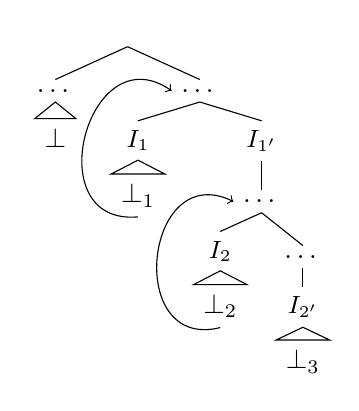
\begin{tikzpicture}
    \tikzset{level distance=20pt, sibling distance=10pt} \Tree [.$$
    [. $\dots$ \edge[roof]; \node(C0) {$\bot$};] [. \node(B1){$\dots$}; [. {\small $I_1$} \edge[roof]; \node(C1) {$\bot_1$}; ] [. {\small $I_{1'}$} [. \node(B2){$\dots$}; [.{\small $I_2$} \edge[roof];\node(C2) {$\bot_2$};]
                                                                                                                      [.$\dots$ [.{\small $I_{2'}$} \edge[roof]; \node(C3) {$\bot_3$};]]]
]]]
]]
    \draw[->, bend left=110, looseness=2] (C1.south) to (B1.west);
    \draw[->, bend left=110, looseness=2] (C2.south) to (B2.west);
  \end{tikzpicture}

  \caption{Example of instance dismissal}
  \label{fig:inst-dismissal}
\end{figure}

Consider in Figure~\ref{fig:inst-dismissal} an example of instance
dismissal. $I_1$ marks an instantiation happening at level $1$, in
which all clauses from the original formula are considered for
instantiation. Those lead to a conflict and a backtrack to a point
before $I_1$, which decrements the instantiation level to $0$. All
instances from $I_1$ which were part of the conflict in $\bot_1$ are
promoted to level $0$, the rest kept with level $1$. At $I_{1'}$ only
terms in clauses with level $0$ are indexed. Since subsequently there
is no backtracking to a point before $I_{1'}$, the instantiation level
is increased to $1$. At $I_2$ all clauses of level $1$ are considered,
thus including those produced both in $I_{1}$ and $I_{1'}$. After a
backtrack, the level is decremented to $1$ and the instances
participating in $\bot_2$ are promoted. This way at $I_{2'}$ only the
promoted instances from the previous round are considered. Then the
ground solver reaches a conflict in $\bot_3$ and cannot produce any
more models, concluding unsatisfiability.

% \subsection{Further optimizations}
% \label{sec:optimizations}

% \begin{itemize}
%   \item \textbf{Bitmask for function symbols}: A frequent operation
%   when searching for instantiations modulo a set of equalities is to
%   assess whether a given congruence class has terms unifiable with
%   some nonground term, i.e., there is an {\eunif} for $\bfapp{x}\simeq
%   \bfapp[g]{t}$ if and only if in $[\bfapp[g]{t}]$ there is a term
%   $\bfapp{t'}$, for which a necessary condition is the class having
%   some term with the top symbol ``f''. Therefore we have implemented a
%   fast check for whether a given class has a specific symbol. Function
%   symbols are associated to a power of 2 as its mask, up to $2^{64}$,
%   all others being associated to $0$. If a given symbol has a nonzero
%   mask it can be determined if a class has terms with that symbol in
%   $\O(1)$, ruling out unification attempts if the symbol is not
%   present. For the symbols beyond the threshold the whole term index
%   must be traversed, but as the indexes are sorted by congruence class
%   this amounts for a binary search for the respective class.

%   \item \textbf{Memoization}: We store the results of {\euni}s
%   attempts to avoid (usually expensive) re-computations. This is
%   particularly useful when looking for unifiers for, e.g.,
%   $\bfapp{x}\simeq \bfapp[g]{y}$ in which both ``\emph{f}'' and
%   ``\emph{g}'' have large term indexes. These ``unification
%   jobs''\smarginpar{This should have been defined upstream} are
%   indexed by the polarity ($\top$ indicates that a substitution must
%   be found that make the two terms congruent, while $\bot$ that they
%   should be made disequal) and the participating terms, such that for
%   the above example we would have $\langle\bfapp{x}, \bfapp[g]{y},
%   \top\rangle$.

%   \item \textbf{Instances trie}: instantiations are kept in a
%   \emph{trie} data structure for each quantified formula. Each node
%   represents the ground term associated to a variable, in order from
%   the first to the last bound variable. Terms are not kept modulo
%   congruence classes, since this information may change between
%   instantiation cycles, according to the current model. This allows a
%   fast check to whether an instantiation is redundant, which is often
%   the case with instantiations produced by triggers.
% \end{itemize}

\section{Experiments}
\label{sec:experiments}

The above techniques have been implemented in the SMT solver
{\verit}~\cite{Bouton2009}, which previously offered support for
quantified formulas solely through na\"ive trigger instantiation,
without further optimizations\footnote{A development version is
  available at
  \url{http://www.loria.fr/~hbarbosa/veriT-ccfv.tar.gz}}. The
evaluation was made on the ``UF'', ``UFLIA'', ``UFLRA'' and ``UFIDL''
categories of SMT-LIB~\cite{Barrett2010}, which have $10,495$
benchmarks annotated as \emph{unsatisfiable}. They consist mostly of
quantified formulas over uninterpreted functions as well as equality
and linear arithmetic. The categories with bit vectors and non-linear
arithmetic are currently not supported by {\verit} and in those in
which uninterpreted functions are not predominant the techniques shown
here are not quite as effective yet. Our experiments were conducted
using machines with 2 CPUs Intel Xeon E5-2630 v3, 8 cores/CPU, 126GB
RAM, 2x558GB HDD. The timeout is set for 30 seconds, since our goal is
evaluating SMT solvers as backends of verification and ITP platforms,
which require fast answers.

% In the scatter plots below, each point in the plot represents a
% benchmark, while each axis represents the CPU time, in seconds, that
% the respective solver took to solve it. Points below the diagonal show
% that the solver in the $y$-axis is faster, and vice-versa. Points on
% the opposite edge of an axis represent problems solved exclusively by
% the respective solver.

The different configurations of {\verit} are identified in this
section according to which techniques they have activated:
\begin{itemize}
  \item {\verit}: the solver relying solely on na\"ive trigger instantiation;
  \item {\verit}\_i: the solver with {\ccfv} and the signature table
  indexed;
  \item {\verit}\_ig: besides the above, uses the goal-oriented search
  for conflicting instances;
  \item {\verit}\_igd: does the term indexing from the SAT solver and
  uses the goal-oriented search and instance dismissal.
\end{itemize}

Figure~\ref{fig:sfig1} shows the big impact of the handling of
instantiation by {\ccfv}: {\verit}\_i is significantly faster and
solves 326 problems exclusively, while the old configuration solves
only 32 exclusively. Figure~\ref{fig:sfig2} presents a significant
improvement in terms of problems solved (474 more against 36 less) by
the use of the goal-oriented instantiation, but it also shows a less
clear gain of time. Besides the natural chaotic behavior of trigger
instantiation, we believe this is due to the more expensive search
performed: trying to falsify quantified formulas and handling {\euni},
which, in the context of SMT, has a much bigger search space than
simply performing {\ematch} for pattern-matching instantiation. Not
always the ``better quality'' of the conflicting instances offsets the
time it took to compute them, which indicates the necessity of trying
to identify beforehand such cases and avoid the more expensive search
when counter-producent.

\begin{figure}[htbp]
\begin{subfigure}{.49\textwidth}
  \centering
  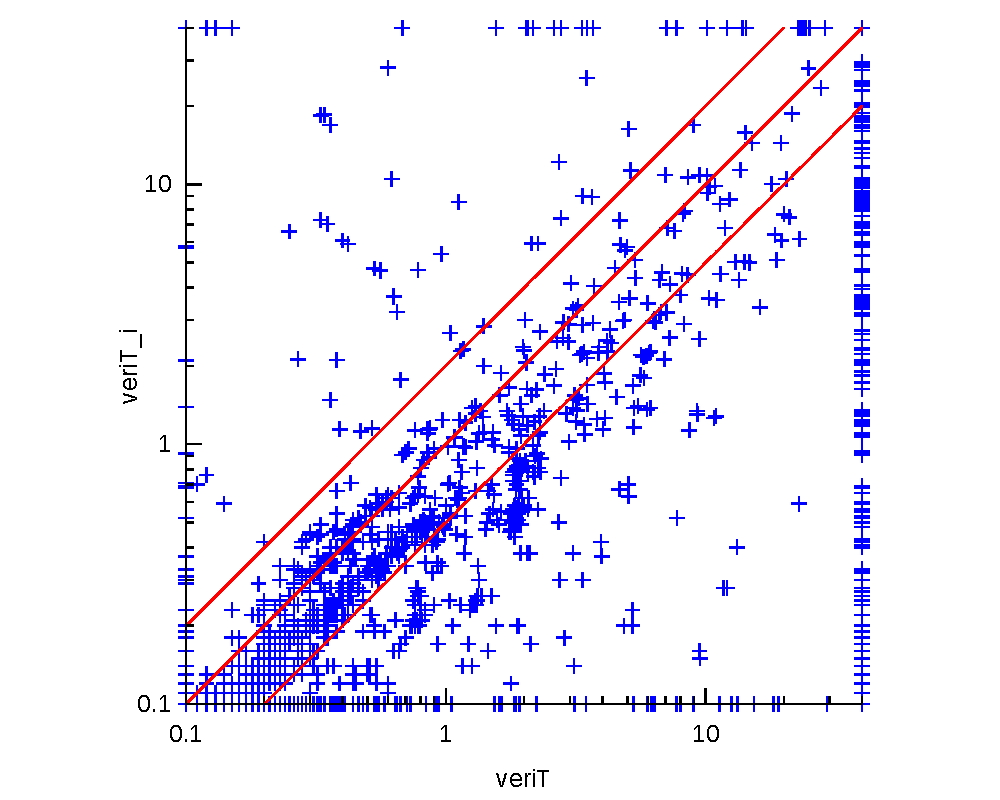
\includegraphics[scale=.42]{i_devel.pdf}
  \caption{Impact of CCFV, without goal-oriented instantiation}
  \label{fig:sfig1}
\end{subfigure}%
\hfill
\begin{subfigure}{.49\textwidth}
  \centering
  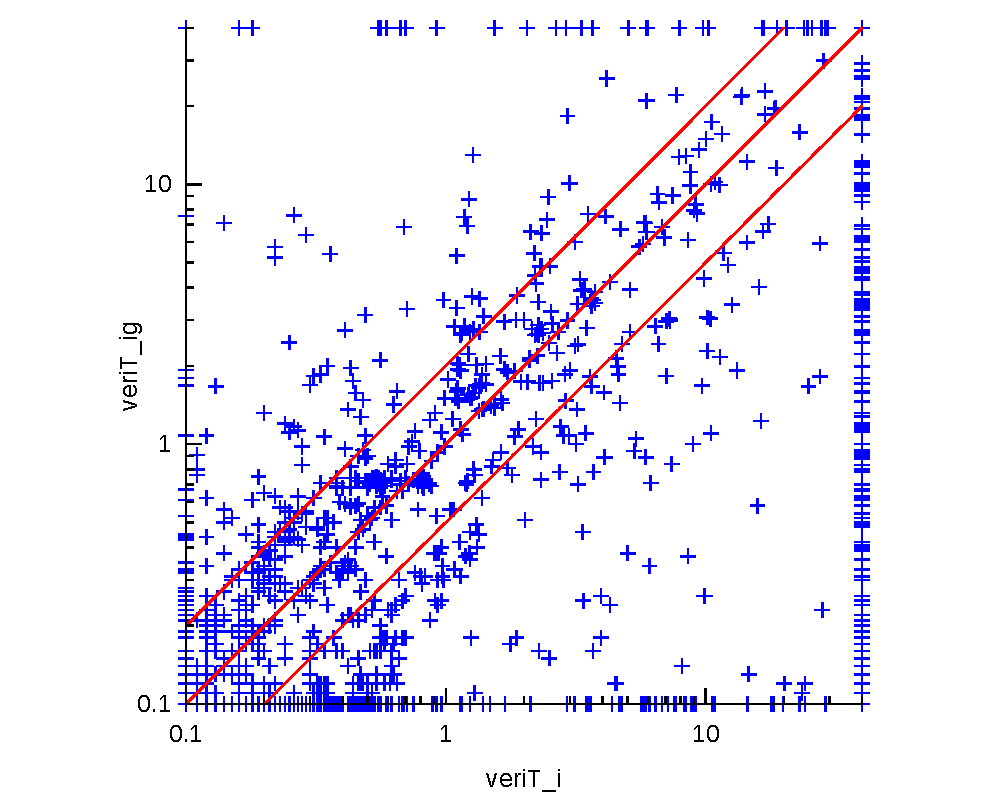
\includegraphics[scale=.42]{SIG_i.pdf}
  \caption{Impact of goal-oriented instantiation}
  \label{fig:sfig2}
\end{subfigure}
\caption{Comparisons of new term indexing, CCFV and goal-oriented search}
\label{fig:fig1}
\end{figure}

\begin{table}[htbp]
  \centering
  \begin{tabular}{|l|l|l|l|l|l|l|l|}
    \hline
    Logic & Class & CVC4 & Z3 & veriT\_igd & veriT\_ig & veriT\_i&veriT\\
    \hline
    \multirow{2}{*}{UF}&grasshopper&410&418&431&\textbf{437}&418&413\\
          &sledgehammer&\textbf{1412}&1249&1293&1272&1134&1066\\
    \hline
    UFIDL&all&61&\textbf{62}&56&58&58&58\\
    \hline
    \multirow{5}{*}{UFLIA}&boogie&841&\textbf{852}&722&681&660&661\\
          &sexpr&15&\textbf{26}&15&7&5&5\\
          &grasshopper&320&341&356&\textbf{367}&340&335\\
          &sledgehammer&\textbf{1892}&1581&1781&1778&1620&1569\\
          &simplify&770&\textbf{831}&797&803&735&690\\
          &simplify2&2226&\textbf{2337}&2277&2298&2291&2177\\
    \hline
    \multicolumn{2}{|c|}{Total}&\textbf{7947}&7697&7727&7701&7203 &6916\\
    \hline
  \end{tabular}

  \caption{Comparison between instantiation based SMT solvers on SMT-LIB benchmarks}
  \label{tab:comparison}
\end{table}

Our new implementations were also evaluated against the SMT
solvers \textsc{Z3}~\cite{deMoura2008-z3} (version 4.4.2) and
\textsc{CVC4}~\cite{Barrett2011} (version 1.5), both based on
instantiation for handling quantified formulas. The results are
summarized in Table~\ref{tab:comparison}, excluding categories whose
problems are trivially solved by all systems, which leaves $8,701$ for
consideration.

While {\verit}\_ig and {\verit}\_igd solve a similar number of
problems in the same categories (with a small advantage to the
latter), it should be noted that they have quite diverse results
depending on the benchmark (a comparison is shown in
Figure~\ref{fig:fig1} at Appendix A). Each configuration solves
$\approx 150$ problems exclusively. This indicates the potential to
use both the term indexes, from the signature table and from the SAT solver
model with instance dismissal, during the solving.

Regarding overall performance, \textsc{CVC4} solves the most problems,
being the more robust SMT solver for instantiation and also applying a
goal-oriented search for conflicting instances. Both configurations of
{\verit} solve approximately the same number of problems as
\textsc{Z3}, although mostly because of the better performance on the
\emph{sledgehammer} benchmarks, which have less theory symbols. There
are 124 problems solved by {\verit}\_igd that neither \textsc{CVC4} nor
\textsc{Z3} solve, while {\verit}\_ig solves 115 that neither of these
two do.

Figure~\ref{fig:fig2} shows how the better {\verit} configuration,
with the goal-oriented search and instance dismissal, performs against
the other solvers. There are many problems solved exclusively by each
system, which indicates the benefit of combining {\verit} with those
systems them in a portfolio when trying to quickly solve a particular
problem: while \textsc{CVC4} alone solves $\approx 92\%$ of the
considered benchmarks in 30s, by giving each of the four compared
systems 7s is enough to solve $\approx 97\%$ of them.

\begin{figure}[htbp]
\begin{subfigure}{.49\textwidth}
  \centering
  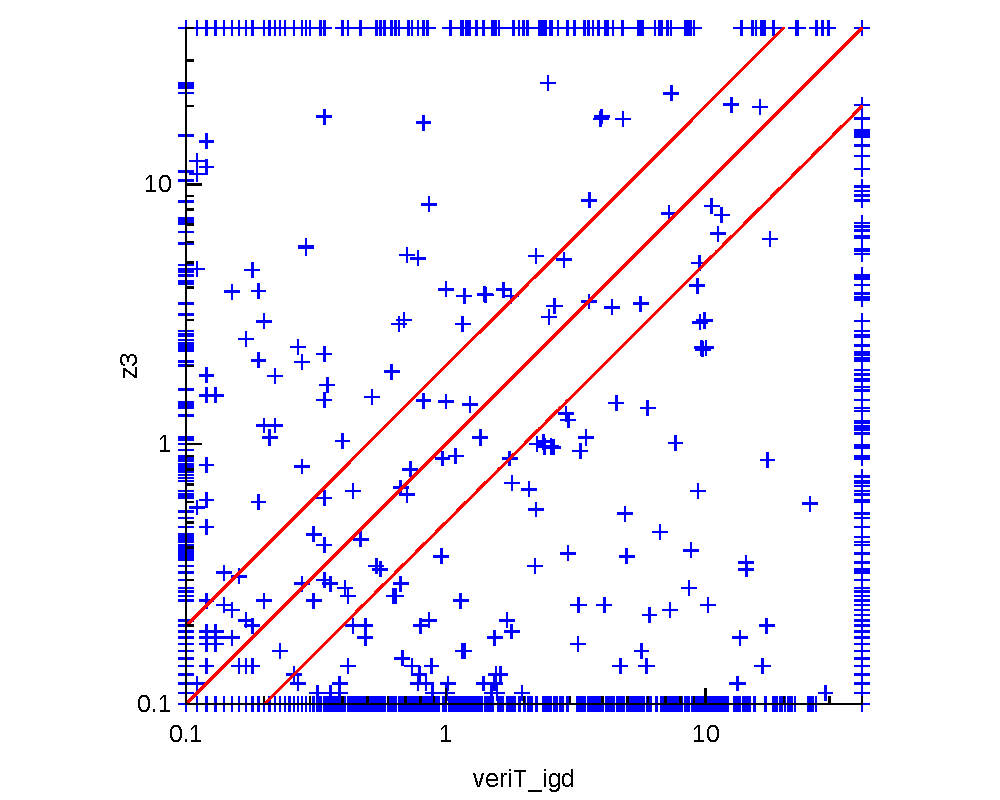
\includegraphics[scale=.42]{z3_del.pdf}
  \caption{\textsc{Z3} vs {\verit}\_igd}
  \label{fig:sfig3}
\end{subfigure}%
\hfill
\begin{subfigure}{.49\textwidth}
  \centering
  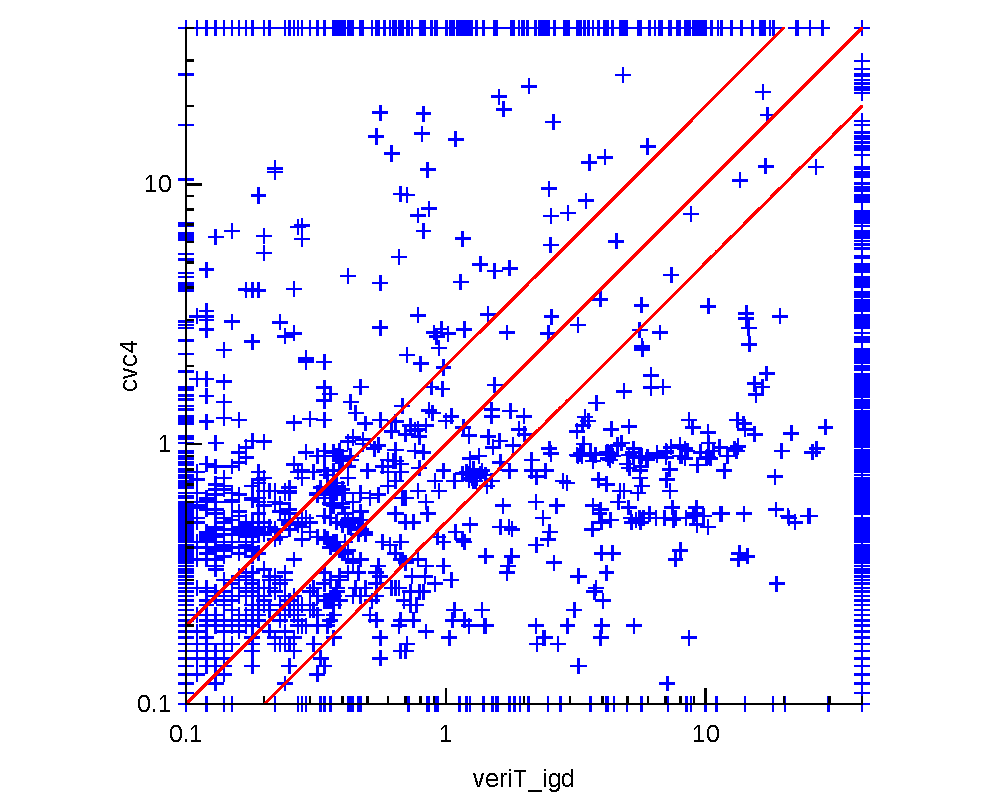
\includegraphics[scale=.42]{cvc4_del.pdf}
  \caption{\textsc{CVC4} vs {\verit}\_igd}
  \label{fig:sfig4}
\end{subfigure}
\caption{Comparisons with SMT solvers}
\label{fig:fig2}
\end{figure}

\section{Conclusion and future work}
\label{sec:conclusion}

There is still room for improvement in our instantiation
framework. Particularly, a better understanding of the instance
dismissal effects is still required. Further analyzing the clauses
activity would lead to a more refined promotion strategy and possibly
better outcomes. Nevertheless, we believe that our preliminary results
are promising.

Regarding the term indexing, besides improving the data structures our
main goal is performing it \emph{incrementally}: by indexing the
literals from the SAT model it is not necessary to thoroughly
recompute the index at each instantiation round. It is sufficient to
simply remove or add terms, as well as update signatures, according to
how the model has changed. The same principle may be applied to the
memoization of ``unification jobs'': an incremental term index would
allow updating the resulting unifiers accordingly, significantly
reducing the instantiation effort over rounds with similar indexes.

Our goal-oriented instantiation has a very limited scope: currently
conflicting instances can only be found when a single quantified
formula is capable of refuting the model. As it has been shown
in~\cite{Reynolds2014} and also in our own experiments this is enough
to provide large improvements over trigger instantiation, but for many
problems it is still insufficient.  We intend to combine {\ccfv} with
the \emph{Connection Calculus}~\cite{Otten2010}, a complete
goal-oriented proof procedure for first-order logic, in an effort for
having a broader approach for deriving conflicting instances. This
would present a much more complex search space than the one our
strategy currently handles. Therefore the trade-off between
expressivity and cost has to be carefully evaluated.

Applying different strategies in a portfolio approach is highly
beneficial for solving more problems, but it could be even more so if
different configurations were to communicate. Attempting
pseudo-concurrent architectures such as described in~\cite{Reger2015}
in {\verit} is certainly worth considering.

\subsubsection*{Acknowledgments} I would like to thank my supervisors
Pascal Fontaine and David D\'{e}harbe for all their help throughout the
development of this work and comments on the article.

Experiments presented in this paper were carried out using the Grid'5000 testbed, supported by a scientific interest group hosted by Inria and including CNRS, RENATER and several Universities as well as other organizations (see https://www.grid5000.fr).


\bibliographystyle{abbrv}
\bibliography{bib}

\newpage

\section*{Appendix A}
\label{sec:appx-A}

\begin{figure}[htbp]
  \centering
  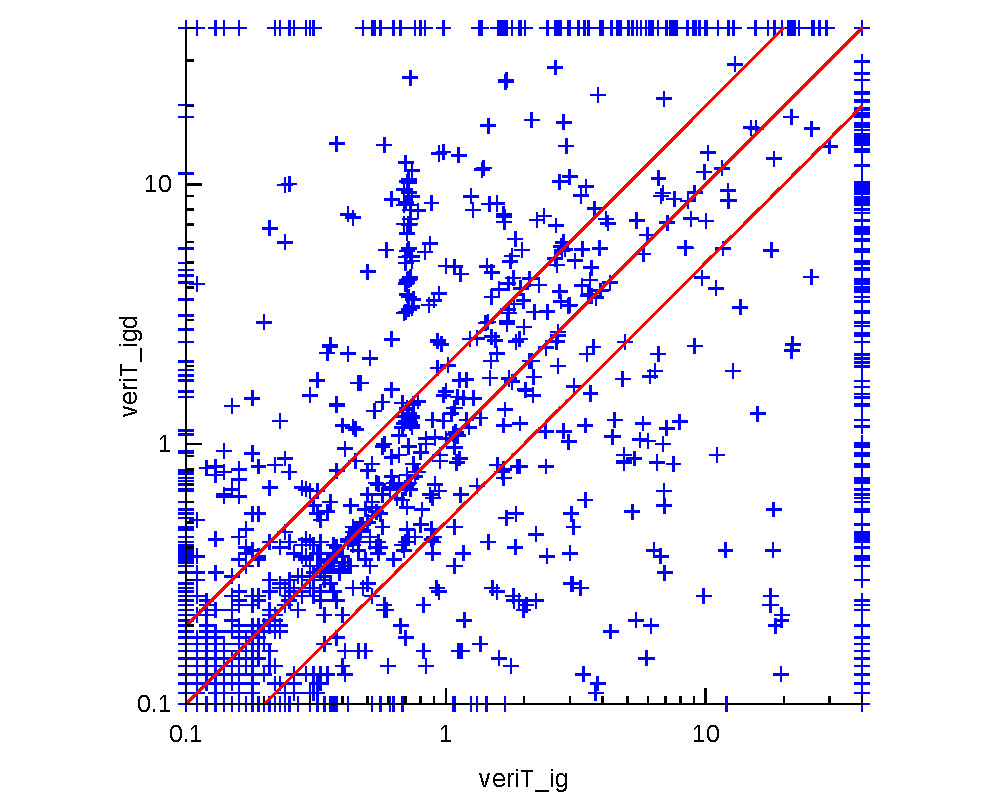
\includegraphics[scale=.5]{del_SIG.pdf}
  \caption{Comparison of the two strategies}
  \label{fig:fig1}
\end{figure}


\end{document}

%%% Local Variables:
%%% mode: latex
%%% TeX-master: t
%%% End:
